\documentclass[tikz]{standalone}
\usepackage{amsmath}
\usepackage{amssymb}
\usepackage{amsfonts}
\usepackage{tikz}
\usetikzlibrary{automata, positioning}
\thispagestyle{empty}
\begin{document}
	

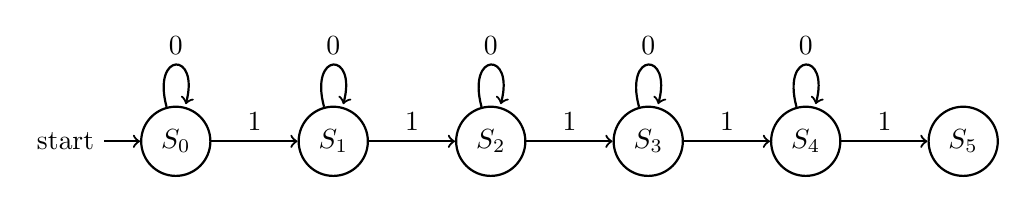
\begin{tikzpicture}[thick,->,node distance=2cm, on grid, auto]
\node[state, initial] (q0) {$S_0$};
\node[state, right of=q0] (q1) {$S_1$}; 
\node[state, right of=q1] (q2) {$S_2$}; 
\node[state, right of=q2] (q3) {$S_3$}; 
\node[state, right of=q3] (q4) {$S_4$}; 
\node[state, right of=q4] (q5) {$S_5$}; 

% Transitions
\foreach \i in {0,1,2,3,4} {
	  \path (q\i) edge[loop above] node {0} (q\i);
}
% Arrows to next state
\foreach \i in {0,1,2,3,4} {
	\pgfmathtruncatemacro{\j}{\i + 1}
	\path (q\i) edge node {1} (q\j);
}
\end{tikzpicture}

\end{document}
